\chapter{Phân tích thiết kế hệ thống}
\section{Khảo sát hiện trạng của hệ thống}
\subsection{Sơ lược về cửa hàng}
Tên cửa hàng: Linh kiện điện tử Nam Hải\par
Trụ sở: 030, đường Hoàng liên, đoạn gần ngân hàng Viettinbank, phường Kim Tân, Thành phố Lào Cai.\par
Cửa hàng Nam Hải được thành lập vào năm 2017 với một cơ sở duy nhất với hai nhân viên kiêm chủ cửa hàng.\par
Cửa hàng chuyên kinh doanh về các loại linh kiện điện tử, vi mạch điều khiển, sạch pin,\dots Đối tượng mà cửa hàng nhắm tới là những người có đam mê về công nghệ, robot, tự động hóa, sinh viên các trường công nghệ.\par
Hiện tại do quy mô vẫn còn nhỏ nên việc quản lý cửa hàng chỉ là thông qua giấy tờ, hóa đơn, sổ sách.
\subsection{Thực trạng cửa hàng}
\begin{itemize}
	\item\textbf{Khâu nhập hàng:}\par
	      \vspace{-1em}
	      \begin{itemize}
		      \item Việc nhập hàng thường là nhập trực tiếp từ các lái buôn bên trung quốc, thường mua sỉ mỗi sản phẩm một lượng nhất định phụ thuộc vào sản phẩm nào bán chạy nhất trong những tháng trước đó.
		      \item Các sản phẩm thường nhập
		            \begin{itemize}
			            \item Các sản phẩm được tiêu thụ mạnh trong tháng, quý
			            \item Các sản phẩm đang nổi theo trend
		            \end{itemize}
		      \item Các yếu tố khi cửa hàng nhập sản phẩm
		            \begin{itemize}
			            \item Ngày nhập
			            \item Số lượng sản phẩm nhập vào
			            \item Nhà phân phối (nếu có)
			            \item Các thông số đi kèm (kích thước, chức năng nổi bật,\dots)
			            \item Gía thành mỗi sản phẩm
		            \end{itemize}
		      \item Các thông số nêu trên đều được cửa hàng lưu lại vào sổ nhập hàng để tiện theo dõi
	      \end{itemize}
	\item\textbf{Khâu bán hàng:}\par
	      \begin{itemize}
		      \item Việc bán hàng được thực hiện một cách trực tiếp, khách hàng sẽ tìm đến tận cửa hàng để chọn mua sản phẩm.
		      \item Thống kê doanh số bán hàng không có được con số chính xác vì khách hàng đến mua không thường xuyên và cũng chỉ mua nhỏ lẻ một vài sản phẩm.
		      \item Thông tin về khách hàng không được lưu lại mà chủ yếu là do mua nhiều nên trở thành khách quen, tùy mỗi khách sẽ có chế độ ưu đãi khác nhau.
	      \end{itemize}
	\item\textbf{Ưu và nhược điểm của phương pháp cũ}\par
	      \begin{itemize}
		      \item\textbf{Ưu điểm:}
		            \begin{itemize}
			            \item Khâu nhập hàng và bán hàng diễn ra nhanh chóng.
			            \item Tiền mua bán được trao tận tay nên không phải lo những khoản phí cho bên thứ ba
		            \end{itemize}
		      \item\textbf{Nhược điểm:}
		            \begin{itemize}
			            \item Giá sản phẩm cao hơn giá gốc vì tốn tiền mặt bằng
			            \item Khách hàng chủ yếu chỉ là khách quen, cách thức quảng cáo chính là qua truyền tai nhau giữa khách quen với những người khác hay tạo những sự kiện khuyến mãi,\dots Nên không thường xuyên và không được hiệu quả trong việc tìm kiếm khách hàng tiềm năng.
			            \item Thông tin được lưu vào sổ nên việc tính toán và tra lại khá mất thời gian. Việc thống kê thường là theo từng quý (tức ba tháng một)
		            \end{itemize}
	      \end{itemize}
\end{itemize}
\subsection{Khảo sát quy trình}
Từ quá trình khảo sát hệ thống như trên, cửa hàng Nam Hải có mong muốn khắc phục những nhược điểm hiện tại đồng thời đặt vấn đề xây dựng một website nhằm tiếp cập đến những khách hàng tiềm năng khác, thông qua trang web cửa hàng mong muốn:
\begin{itemize}
	\item Giới thiệu các sản phẩm của cửa hàng, giúp khách hàng đặt mua nhanh chóng, thuận lợi.
	\item Hỗ trợ việc nhập xuất thống kê doanh thu, hàng tồn kho
\end{itemize}\par
Một số chức năng cơ bản:
\begin{itemize}
	\item Với khách hàng:
	      \begin{itemize}
		      \item Xem thông tin sản phẩm.
		      \item Đặt mua sản phẩm.
		      \item Tìm kiếm sản phẩm.
		      \item xem lịch sử giao dịch gần đây
	      \end{itemize}
	\item Với chủ shop:
	      \begin{itemize}
		      \item Quản lý sản phẩm
		      \item Quản lý đơn hàng
		      \item Thống kê doanh thu
	      \end{itemize}
\end{itemize}
\newpage
\section{Phân tích và thiết kế hệ thống}
\subsection{Biểu đồ Usecase}
\begin{enumerate}[label=\textbf{\alph*)}]
	\item \textbf{Biểu đồ tổng quát}
	      \begin{figure}[h!]
		      \centering
		      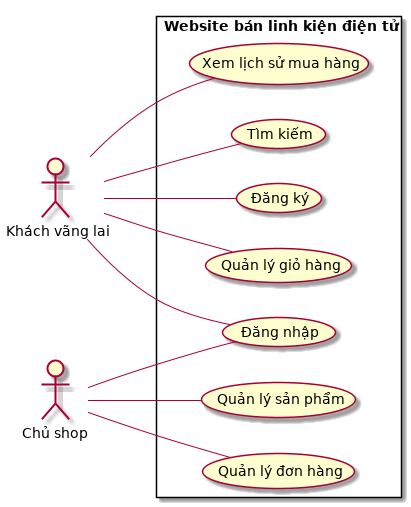
\includegraphics[scale=0.7]{fig/uc_all.png}
		      \caption{Biểu đồ tổng quát}
	      \end{figure}
	      \newpage
	\item \textbf{Biểu đồ phân rã cho tác nhân Khách hàng}
	      \begin{figure}[h!]
		      \centering
		      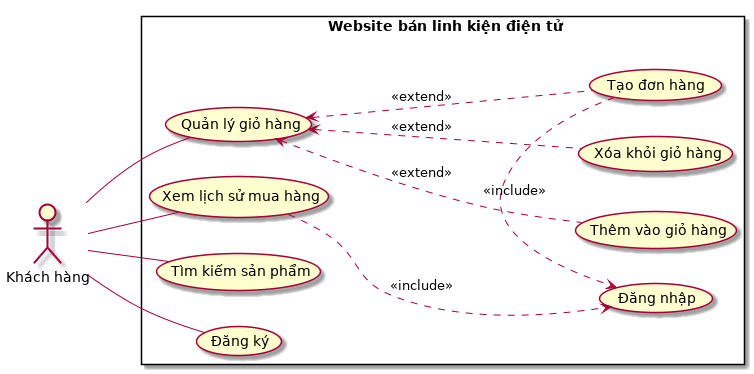
\includegraphics[scale=0.58]{fig/uc_user.png}
		      \caption{Biểu đồ phân rã tác nhân Khách hàng}
	      \end{figure}
	      \newpage
	\item \textbf{Biểu đồ phân rã cho tác nhân Chủ shop}
	      \begin{figure}[h!]
		      \centering
		      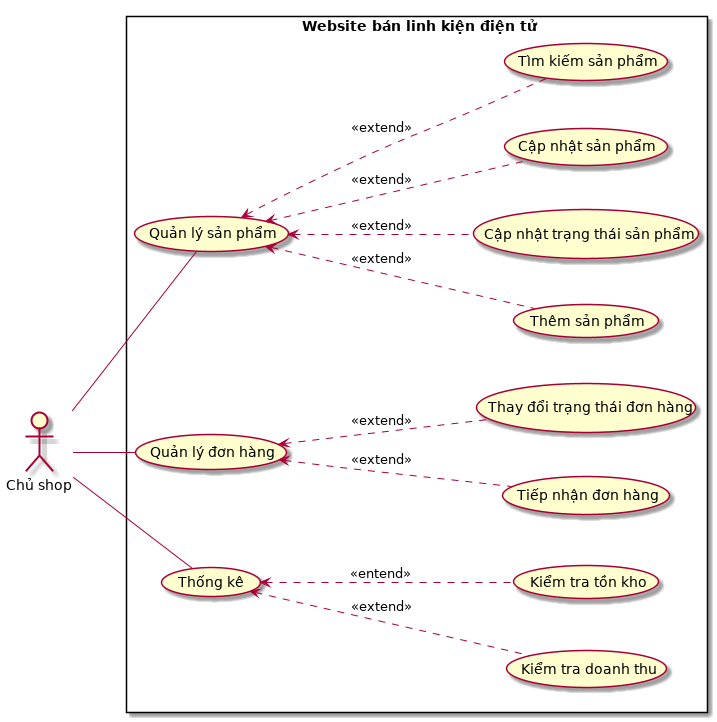
\includegraphics[scale=0.6]{fig/uc_admin.png}
		      \caption{Biểu đồ phân rã tác nhân Chủ shop}
	      \end{figure}
\end{enumerate}
\subsection{Kịch bản cho một số use case chính}
\begin{boxed}
	\textbf{Use case 1:} Đăng nhập                                                             \\
	\textbf{Tác nhân chính:} Khách vãng lai                                                    \\
	\textbf{Mức:} 1                                                                            \\
	\textbf{Tiền điều kiện:} Không có                                                          \\
	\textbf{Luồng kịch bản chính:}                                                             \\
    \begin{enumerate}
    	\vspace{-2em}
    	\itemsep-0.5em
    	\item Khách vãng lai nhập tài khoản và mật khẩu của mình và bấm đăng nhập.
    	\item Khách vãng lai nhấn nút đăng nhập
    	\item Hệ thống xác thực thông tin Khách vãng lai nhập vào.
    	\item Hệ thống tiến hàng đăng nhập
    	\item Hệ thống điều hướng và đưa người dùng về trang quản lý phù hợp với từng loại tài khoản (Trang quản lý thông tin cá nhân đối với Người dùng thông thường, trang quản lý đối với chủ cửa hàng).
    	\vspace{-1em}
    \end{enumerate}
	\textbf{Ngoại lệ:}                                                                         \\
	\hspace{1em}2.a: Thông tin khách vãng lai nhập vào không chính xác                         \\
	\hspace{2.5em}.1 Khách vãng lai có thể chọn đăng ký tài khoản                              \\
	\textbf{Đảm bảo thành công:} Khách vãng lai đăng nhập thành công và được coi là Người dùng \\
	\textbf{Kích hoạt:} Khách vãng lai chọn chức năng đăng nhập
\end{boxed}

\begin{boxed}
	\textbf{Use case 2:} Đăng ký                                                               \\
	\textbf{Tác nhân chính:} Khách vãng lai                                                    \\
	\textbf{Mức:} 1                                                                            \\
	\textbf{Tiền điều kiện:} Không có                                                          \\
	\textbf{Luồng kịch bản chính:}                                                             \\
	\begin{enumerate}
		\vspace{-2em}
		\itemsep-0.5em
		\item Khách vãng lai nhập những thông tin được yêu cầu vào form đăng ký
		\item Khách vãng lai nhấn nút đăng ký
		\item Hệ thống xác thực thông tin Khách vãng lai nhập vào.
		\item Hệ thống điều hướng và đưa người dùng về trang đăng nhập.
		      \vspace{-1em}
	\end{enumerate}
	\textbf{Ngoại lệ:}                                                                         \\
	\hspace{1em}2.a: Khách vãng lai nhập thiếu thông tin hoặc thông tin nhập vào không hợp lệ  \\
	\hspace{2.5em}.1 Hệ thống yêu cầu người dùng nhập lại thông tin                            \\
	\textbf{Đảm bảo thành công:} Khách vãng lai đăng nhập thành công và được coi là Người dùng \\
	\textbf{Kích hoạt:} Khách vãng lai chọn chức năng đăng ký
\end{boxed}

\begin{boxed}
	\textbf{Use case 3:} Thêm sản phẩm vào giỏ hàng                                                \\
	\textbf{Tác nhân chính:} Người dùng                                                            \\
	\textbf{Mức:} 3                                                                                \\
	\textbf{Tiền điều kiện:} Đã thực hiện usecase 1 và là người dùng thông thường                  \\
	\textbf{Luồng kịch bản chính:}                                                                 \\
	\begin{enumerate}
		\vspace{-2em}
		\itemsep-0.5em
		\item Người dùng tìm kiếm và chọn ra sản phẩm mà mình mong muốn
		\item Người dùng chọn xem chi tiết sản phẩm và chọn số lượng sản phẩm muốn mua sau đó bấm thêm vào giỏ hàng
		\item Hệ thống thực hiện thêm thông tin sản phẩm  (id, số lượng, đơn giá) vào giỏ hàng
		\item Hệ thống cập nhật số sản phẩm trong giỏ hàng
		      \vspace{-1em}
	\end{enumerate}
	\textbf{Ngoại lệ:}                                                                             \\
	\hspace{1em}2.a: Sản phẩm hết hàng hoặc ngừng kinh doanh                                       \\
	\hspace{2.5em}.1 Hệ thống ẩn nút Thêm vào giỏ hàng và hiện thông báo với người dùng            \\
	\hspace{1em}3.a: Sản phẩm hết hàng hoặc ngừng kinh doanh                                       \\
	\hspace{2.5em}.1 Nếu sản phẩm đã được thêm từ trước thì hệ thống sẽ chỉ tăng số lượng sản phẩm \\
	\textbf{Đảm bảo thành công:} Thông tin sản phẩm được cập nhật thành công                       \\
	\textbf{Kích hoạt:} Chủ cửa hàng chọn chức năng quản lý sản phẩm
\end{boxed}

\begin{boxed}
	\textbf{Use case 4:} Tạo hóa đơn                                         \\
	\textbf{Tác nhân chính:} Không có                                        \\
	\textbf{Mức:} 3                                                          \\
	\textbf{Tiền điều kiện:} Có ít nhất một sản phẩm trong giỏ hàng          \\
	\textbf{Luồng kịch bản chính:}                                           \\
	\begin{enumerate}
		\vspace{-2em}
		\itemsep-0.5em
		\item Hệ thống kiểm tra, nếu là khách vãng lai thì yêu cầu đăng nhập
		\item Người dùng thay đổi địa chỉ ship hàng và thêm ghi chú (nếu cần) sau đó bấm đặt hàng
		\item Hệ thống thêm đơn hàng vào CSDL và đưa ra thông báo đặt hàng thành công
		      \vspace{-1em}
	\end{enumerate}
	\textbf{Ngoại lệ:}                                                       \\
	\hspace{1em}2.a: Địa chỉ ship để trống                                   \\
	\hspace{2.5em}.1 Hệ thống thông báo lỗi tới người dùng                   \\
	\textbf{Đảm bảo thành công:} Thông tin sản phẩm được cập nhật thành công \\
	\textbf{Kích hoạt:} Chủ cửa hàng chọn chức năng quản lý sản phẩm
\end{boxed}

\begin{boxed}
	\textbf{Use case 5:} Cập nhật thông tin sản phẩm                          \\
	\textbf{Tác nhân chính:} Chủ cửa hàng                                     \\
	\textbf{Mức:} 3                                                           \\
	\textbf{Tiền điều kiện:} Đã đăng nhập vào hệ thống với tài khoản quản trị \\
	\textbf{Luồng kịch bản chính:}                                            \\
	\begin{enumerate}
		\vspace{-2em}
		\itemsep-0.5em
		\item Chủ cửa hàng tìm kiếm sản phầm muốn sửa hoặc chọn tại danh sách mới thêm và bấm sửa
		\item Chủ cửa hàng nhập thông tin mới cập nhật
		\item Chủ cửa hàng bấm nút đăng nhập
		\item Hệ thống kiểm tra thông tin người dùng nhập vào và cập nhật Lên CSDL
		\item Hệ thống điều hướng và đưa người dùng về trang Quản lý thông tin.
		      \vspace{-1em}
	\end{enumerate}
	\textbf{Ngoại lệ:}                                                        \\
	\hspace{1em}6.a: Thông tin Chủ cửa hàng nhập vào không hợp lệ             \\
	\hspace{2.5em}.1 Hệ thống báo lỗi và không cập nhật thông tin lên CSDL    \\
	\textbf{Đảm bảo thành công:} Thông tin sản phẩm được cập nhật thành công  \\
	\textbf{Kích hoạt:} Chủ cửa hàng chọn chức năng quản lý sản phẩm
\end{boxed}
\newpage
\subsection{Biểu đồ lớp}
\begin{enumerate}[label=\textbf{\alph*)}]
	\item Lớp đăng ký
	      \begin{figure}[h!]
		      \centering
		      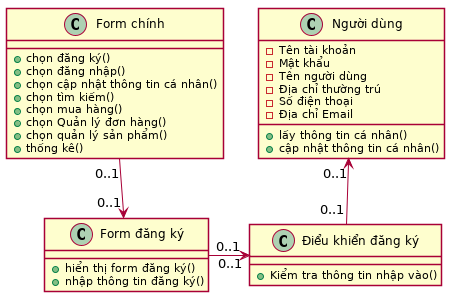
\includegraphics[scale=0.7]{fig/class_dangky.png}
		      \caption{Lớp đăng ký}
	      \end{figure}
	\item Lớp đăng nhập
	      \begin{figure}[h!]
		      \centering
		      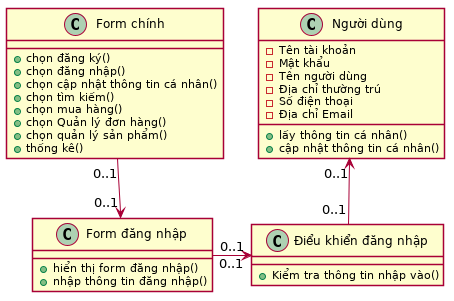
\includegraphics[scale=0.7]{fig/class_dangnhap.png}
		      \caption{Lớp đăng nhập}
	      \end{figure}
          \newpage
	\item Lớp cập nhật thông tin cá nhân
	      \begin{figure}[h!]
		      \centering
		      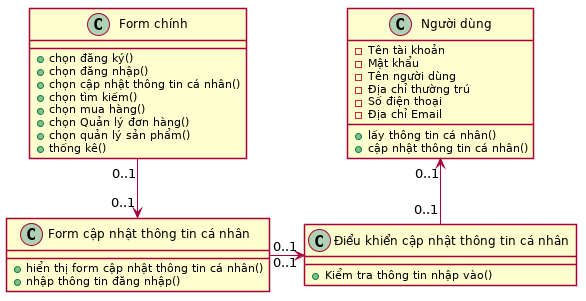
\includegraphics[scale=0.7]{fig/class_update_info.png}
		      \caption{Lớp cập nhật thông tin cá nhân}
	      \end{figure}
	\item Lớp tìm kiếm
	      \begin{figure}[h!]
		      \centering
		      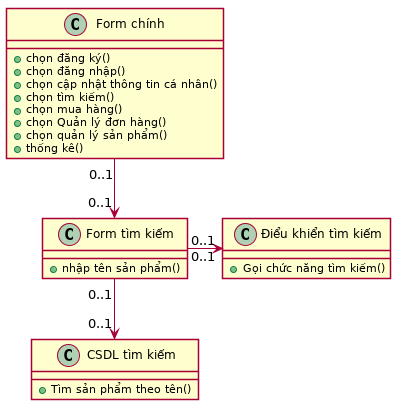
\includegraphics[scale=0.7]{fig/class_timkiem.png}
		      \caption{Lớp tìm kiếm}
	      \end{figure}
          \newpage
	\item Lớp mua hàng
	      \begin{figure}[h!]
		      \centering
		      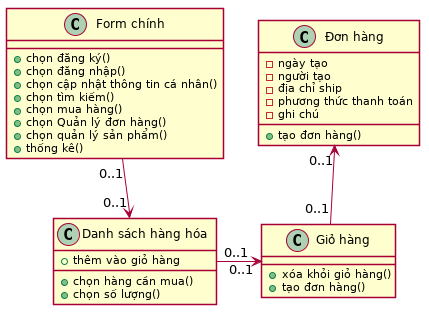
\includegraphics[scale=0.7]{fig/class_muahang.png}
		      \caption{Lớp mua hàng}
	      \end{figure}
	\item Lớp quản lý đơn hàng
	      \begin{figure}[h!]
		      \centering
		      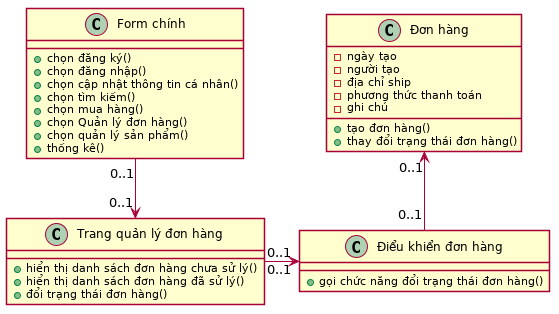
\includegraphics[scale=0.7]{fig/class_qldonhang.png}
		      \caption{Lớp quản lý đơn hàng}
	      \end{figure}
          \newpage
	\item Lớp quản lý sản phẩm
	      \begin{figure}[h!]
		      \centering
		      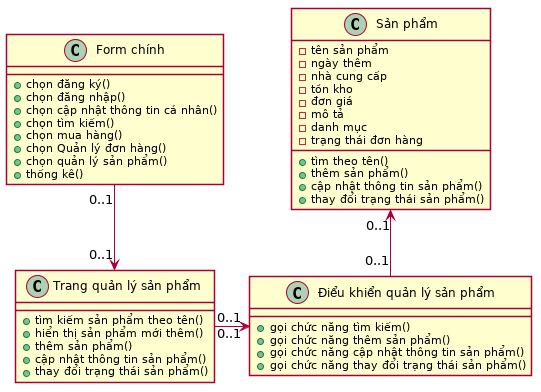
\includegraphics[scale=0.7]{fig/class_quanlysanpham.png}
		      \caption{Lớp quản lý sản phẩm}
	      \end{figure}
	\item Lớp thống kê
	      \begin{figure}[h!]
		      \centering
		      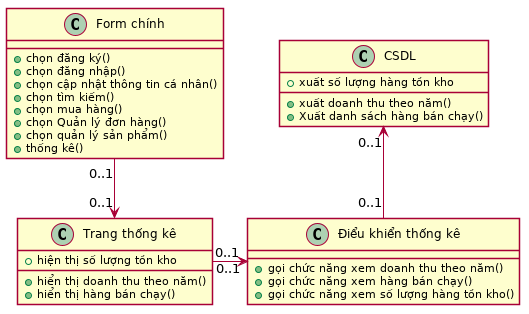
\includegraphics[scale=0.7]{fig/class_thongke.png}
		      \caption{Lớp thống kê}
	      \end{figure}
\end{enumerate}
\newpage
\subsection{Biểu đồ hoạt động}
\begin{enumerate}[label=\textbf{\alph*)}]
	\item Biểu đồ hoạt động cho chức năng đăng nhập
	      \begin{figure}[h!]
		      \centering
		      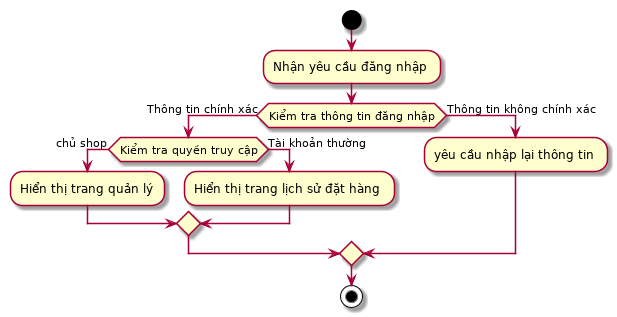
\includegraphics[scale=0.7]{fig/a_login.png}
		      \caption{Biểu đồ hoạt động cho chức năng đăng nhập}
	      \end{figure}
	\item Biểu đồ hoạt động cho chức năng thêm vào giỏ hàng
	      \begin{figure}[h!]
		      \centering
		      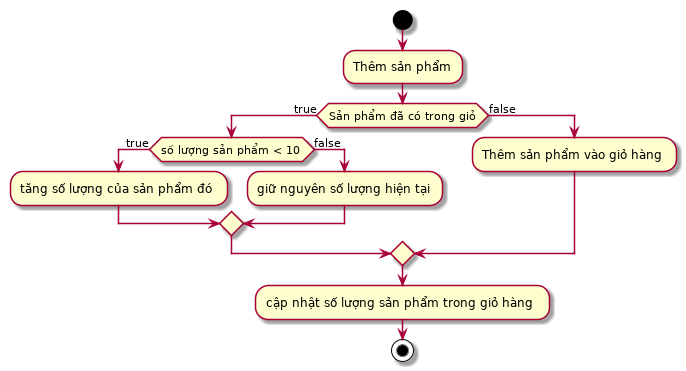
\includegraphics[scale=0.7]{fig/a_cart.png}
		      \caption{Biểu đồ hoạt động cho chức năng thêm vào giỏ hàng}
	      \end{figure}
          \newpage
	\item Biểu đồ hoạt động cho chức năng thanh toán
	      \begin{figure}[h!]
		      \centering
		      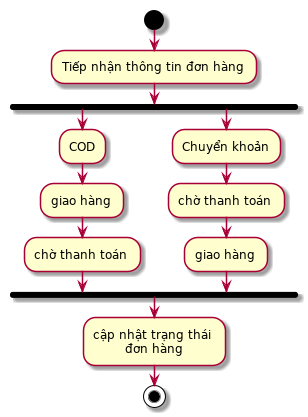
\includegraphics[scale=0.7]{fig/a_order.png}
		      \caption{Biểu đồ hoạt động cho chức năng thanh toán}
	      \end{figure}
\end{enumerate}
\newpage
\subsection{Biểu đồ tuần tự cho một số chức năng chính}
\begin{enumerate}[label=\textbf{\alph*)}]
	\item Chức năng lấy thông tin sản phẩm
	      \begin{figure}[h!]
		      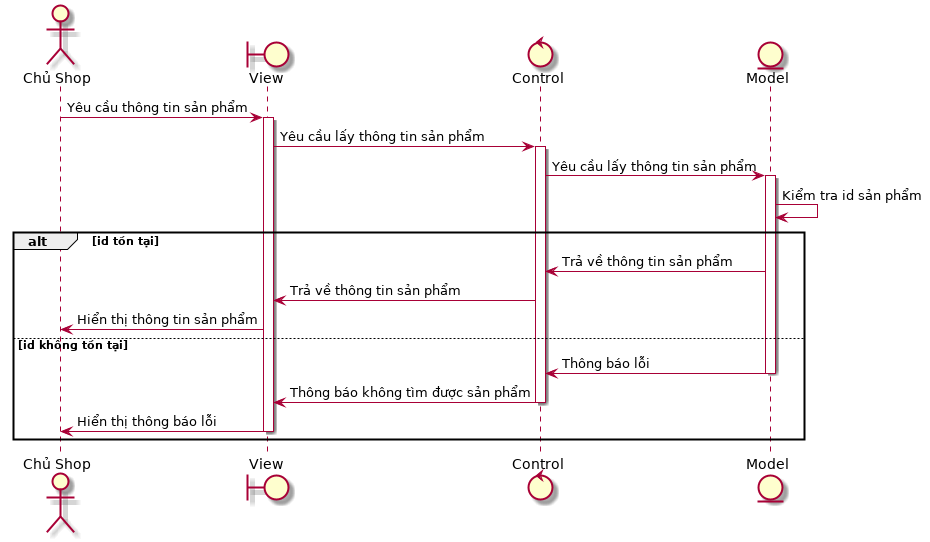
\includegraphics[scale=0.5]{fig/s_get_product_info.png}
		      \caption{Biểu đồ tuần tự cho chức năng lấy thông tin sản phẩm}
	      \end{figure}

	\item Chức năng cập nhật thông tin sản phẩm
	      \begin{figure}[h!]
		      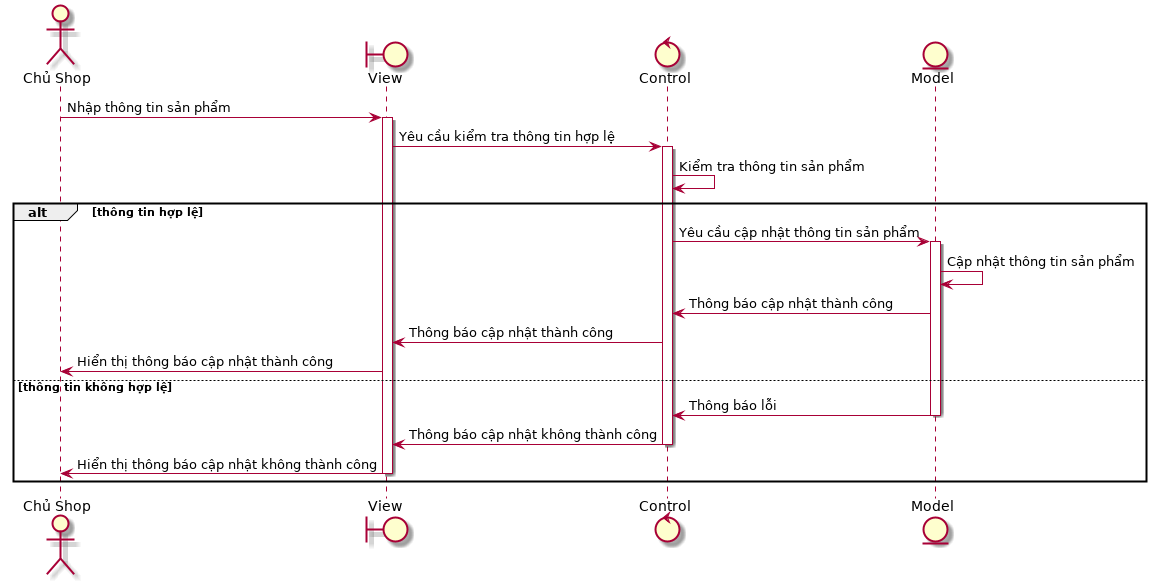
\includegraphics[scale=0.4]{fig/s_update_product_info.png}
		      \caption{Biểu đồ tuần tự cho chức năng cập nhật thông tin sản phẩm}
	      \end{figure}
	\item Chức năng thêm vào giỏ hàng
	      \begin{figure}[h!]
		      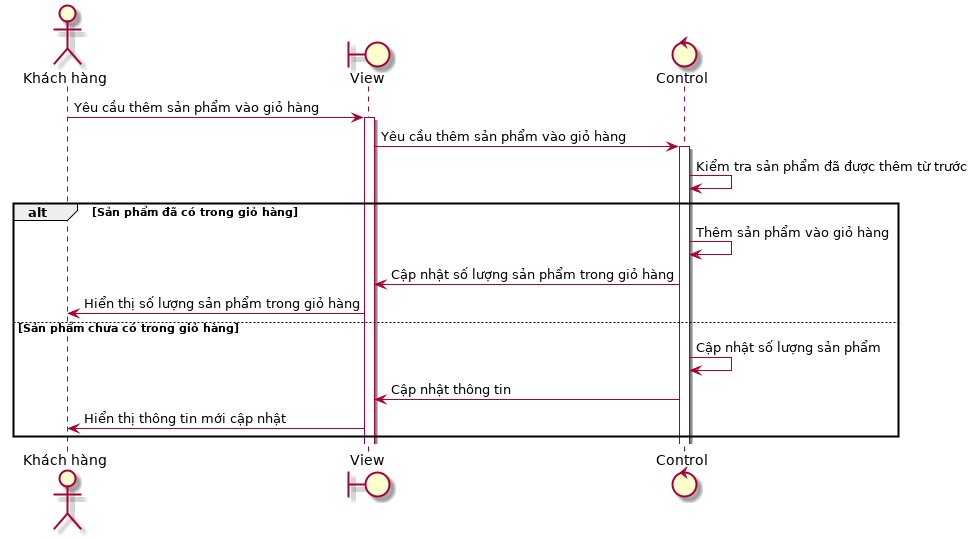
\includegraphics[scale=0.45]{fig/s_add_to_cart.png}
		      \caption{Biểu đồ tuần tự cho chức năng thêm vào giỏ hàng}
	      \end{figure}
\end{enumerate}
\newpage
\subsection{Biểu đồ lớp thực thể}
    \begin{figure}[h!]
        \centering
        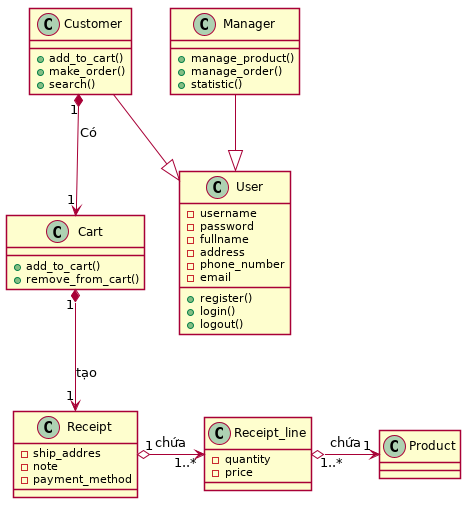
\includegraphics[scale=0.7]{fig/class.png}
        \caption{Biểu đồ lớp thực thể}
    \end{figure}
\newpage
\subsection{Biểu đồ quan hệ thực thể}
\begin{figure}[h!]
	\centering
	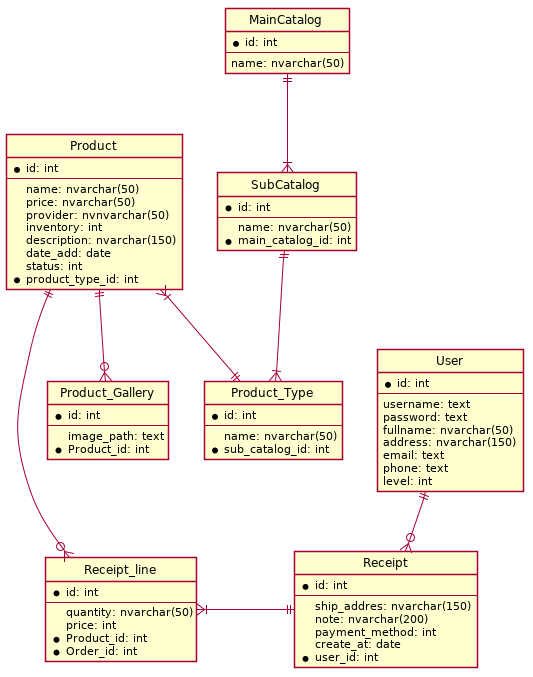
\includegraphics[scale=0.6]{fig/er.png}
	\caption{Biểu đồ quan hệ thực thể}
\end{figure}
\subsection{Biểu đồ triển khai}
\begin{figure}[h!]
	\centering
	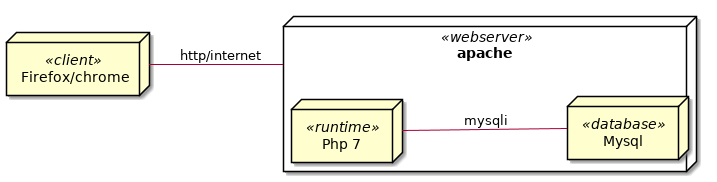
\includegraphics[scale=0.6]{fig/deploy.png}
	\caption{Biểu đồ triển khai}
\end{figure}
\newpage
\section{Một số nguyên mẫu thiết kế trang web}
\begin{enumerate}[label=\textbf{\alph*)}]
    \item Thiết kế trang chủ
        \begin{figure}[h!]
	        \centering
	        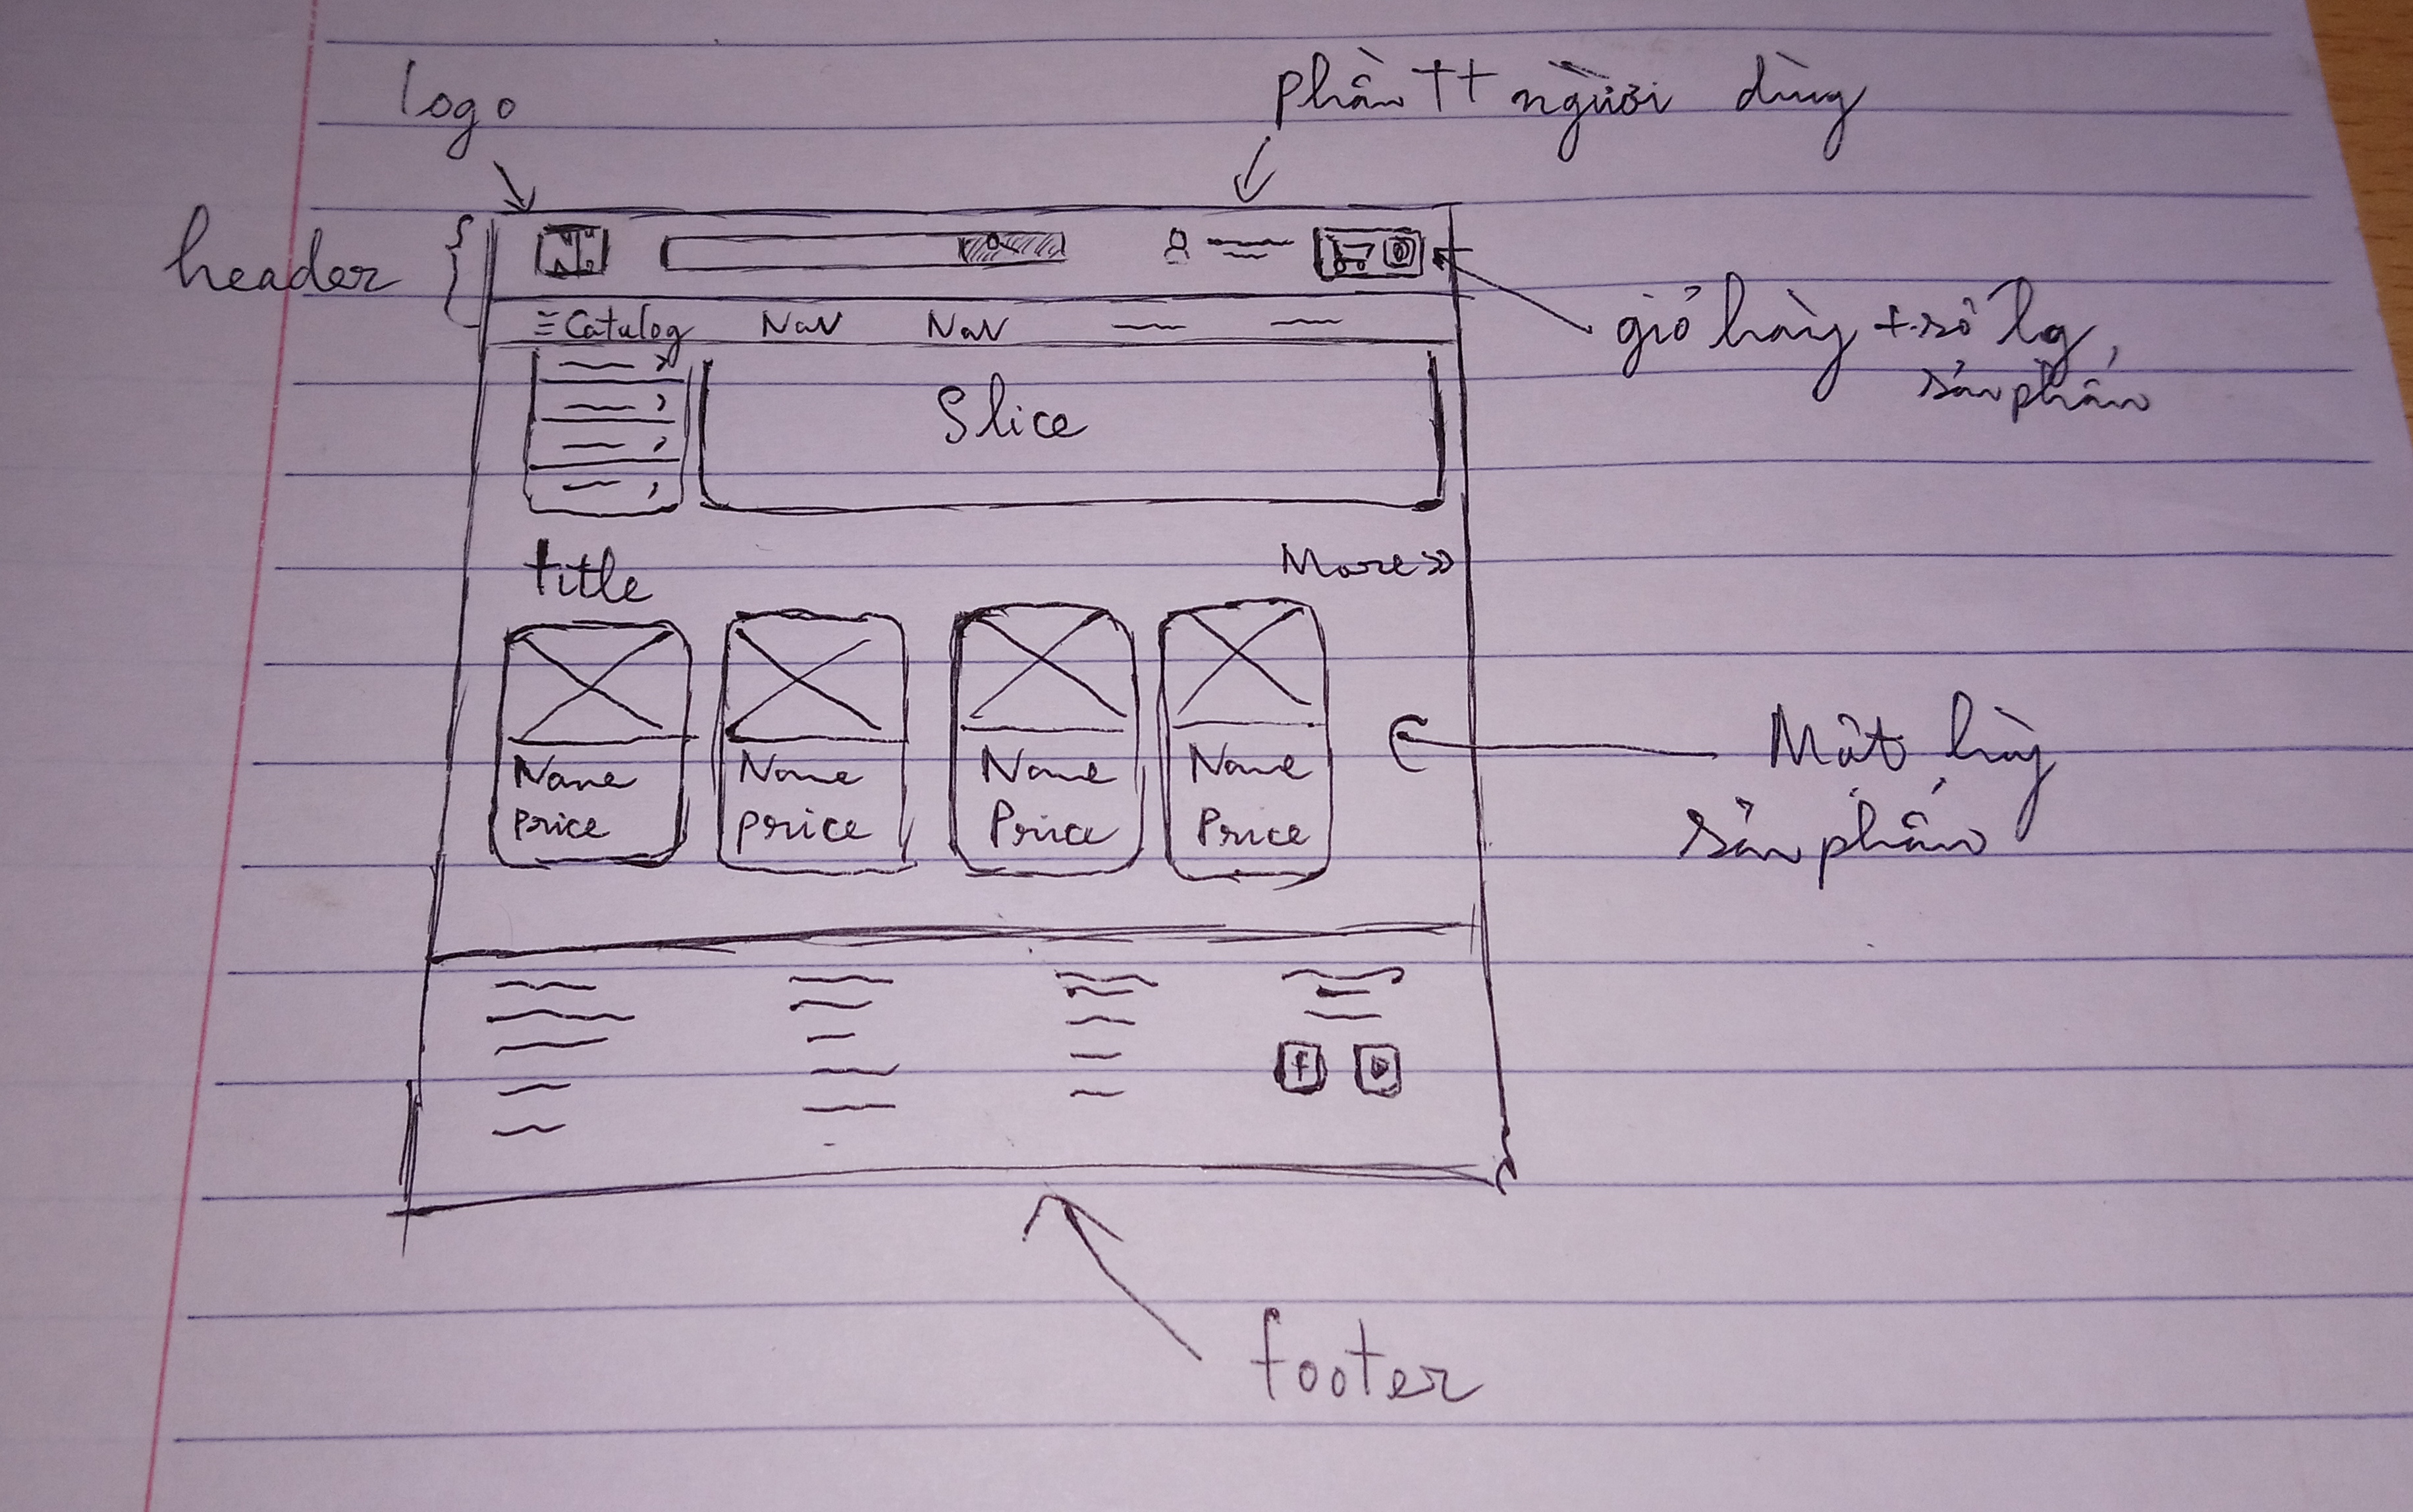
\includegraphics[width=\linewidth]{fig/p_home.jpg}
	        \caption{Nguyên mẫu thiết kế trang chủ}
        \end{figure}
    \item Thiết kế giỏ hàng
        \begin{figure}[h!]
            \centering
            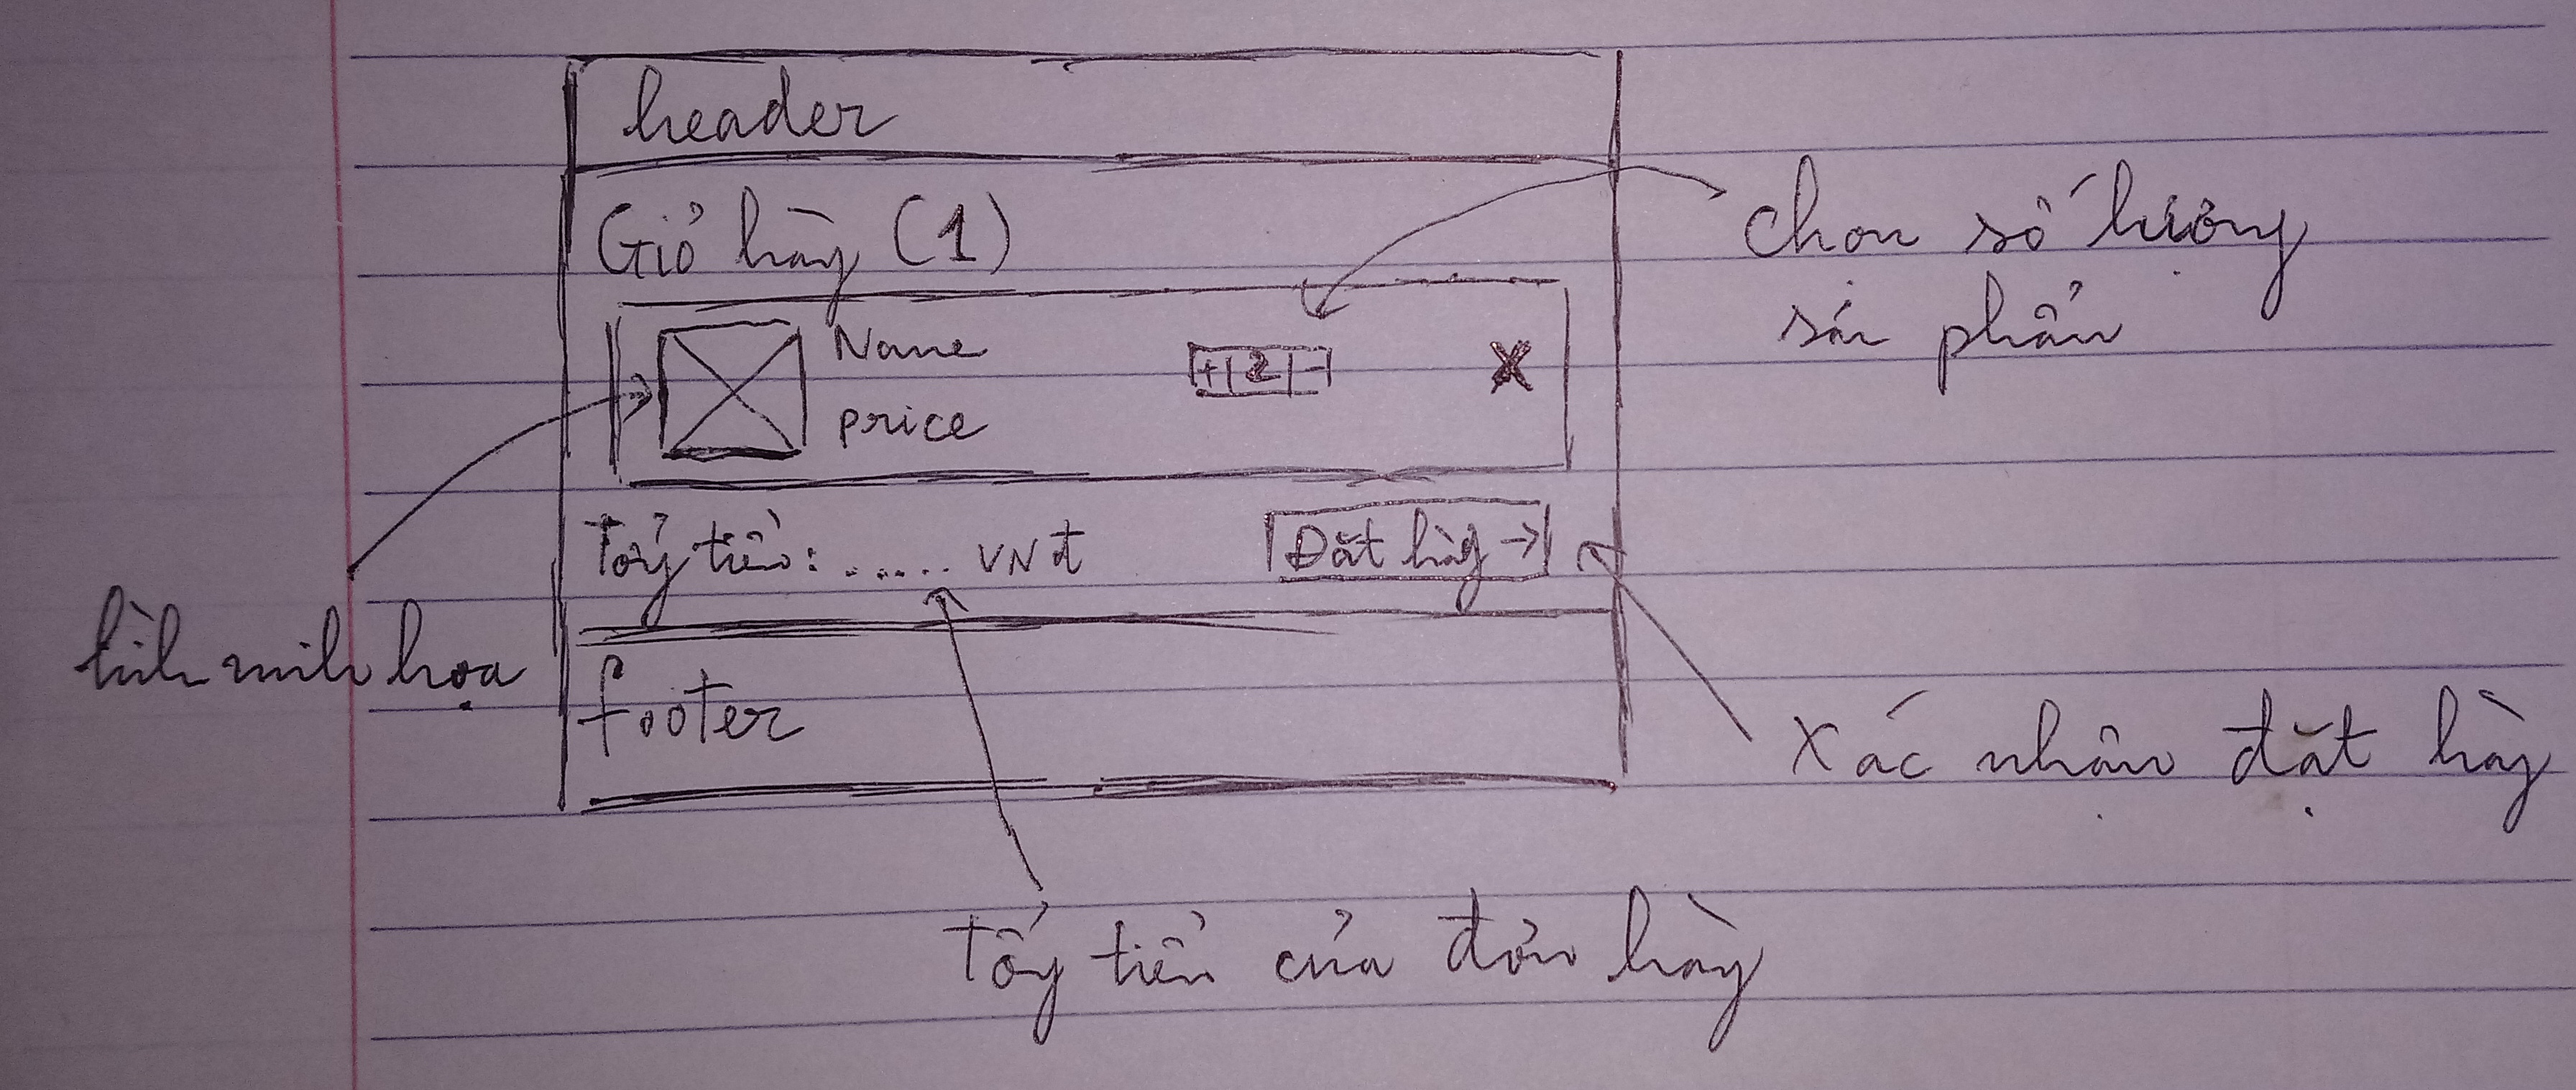
\includegraphics[width=\linewidth]{fig/p_cart.jpg}
            \caption{Nguyên mẫu thiết kế giỏ hàng}
        \end{figure}
    \newpage
    \item Thiết kế trang quản trị
        \begin{figure}[h!]
            \centering
            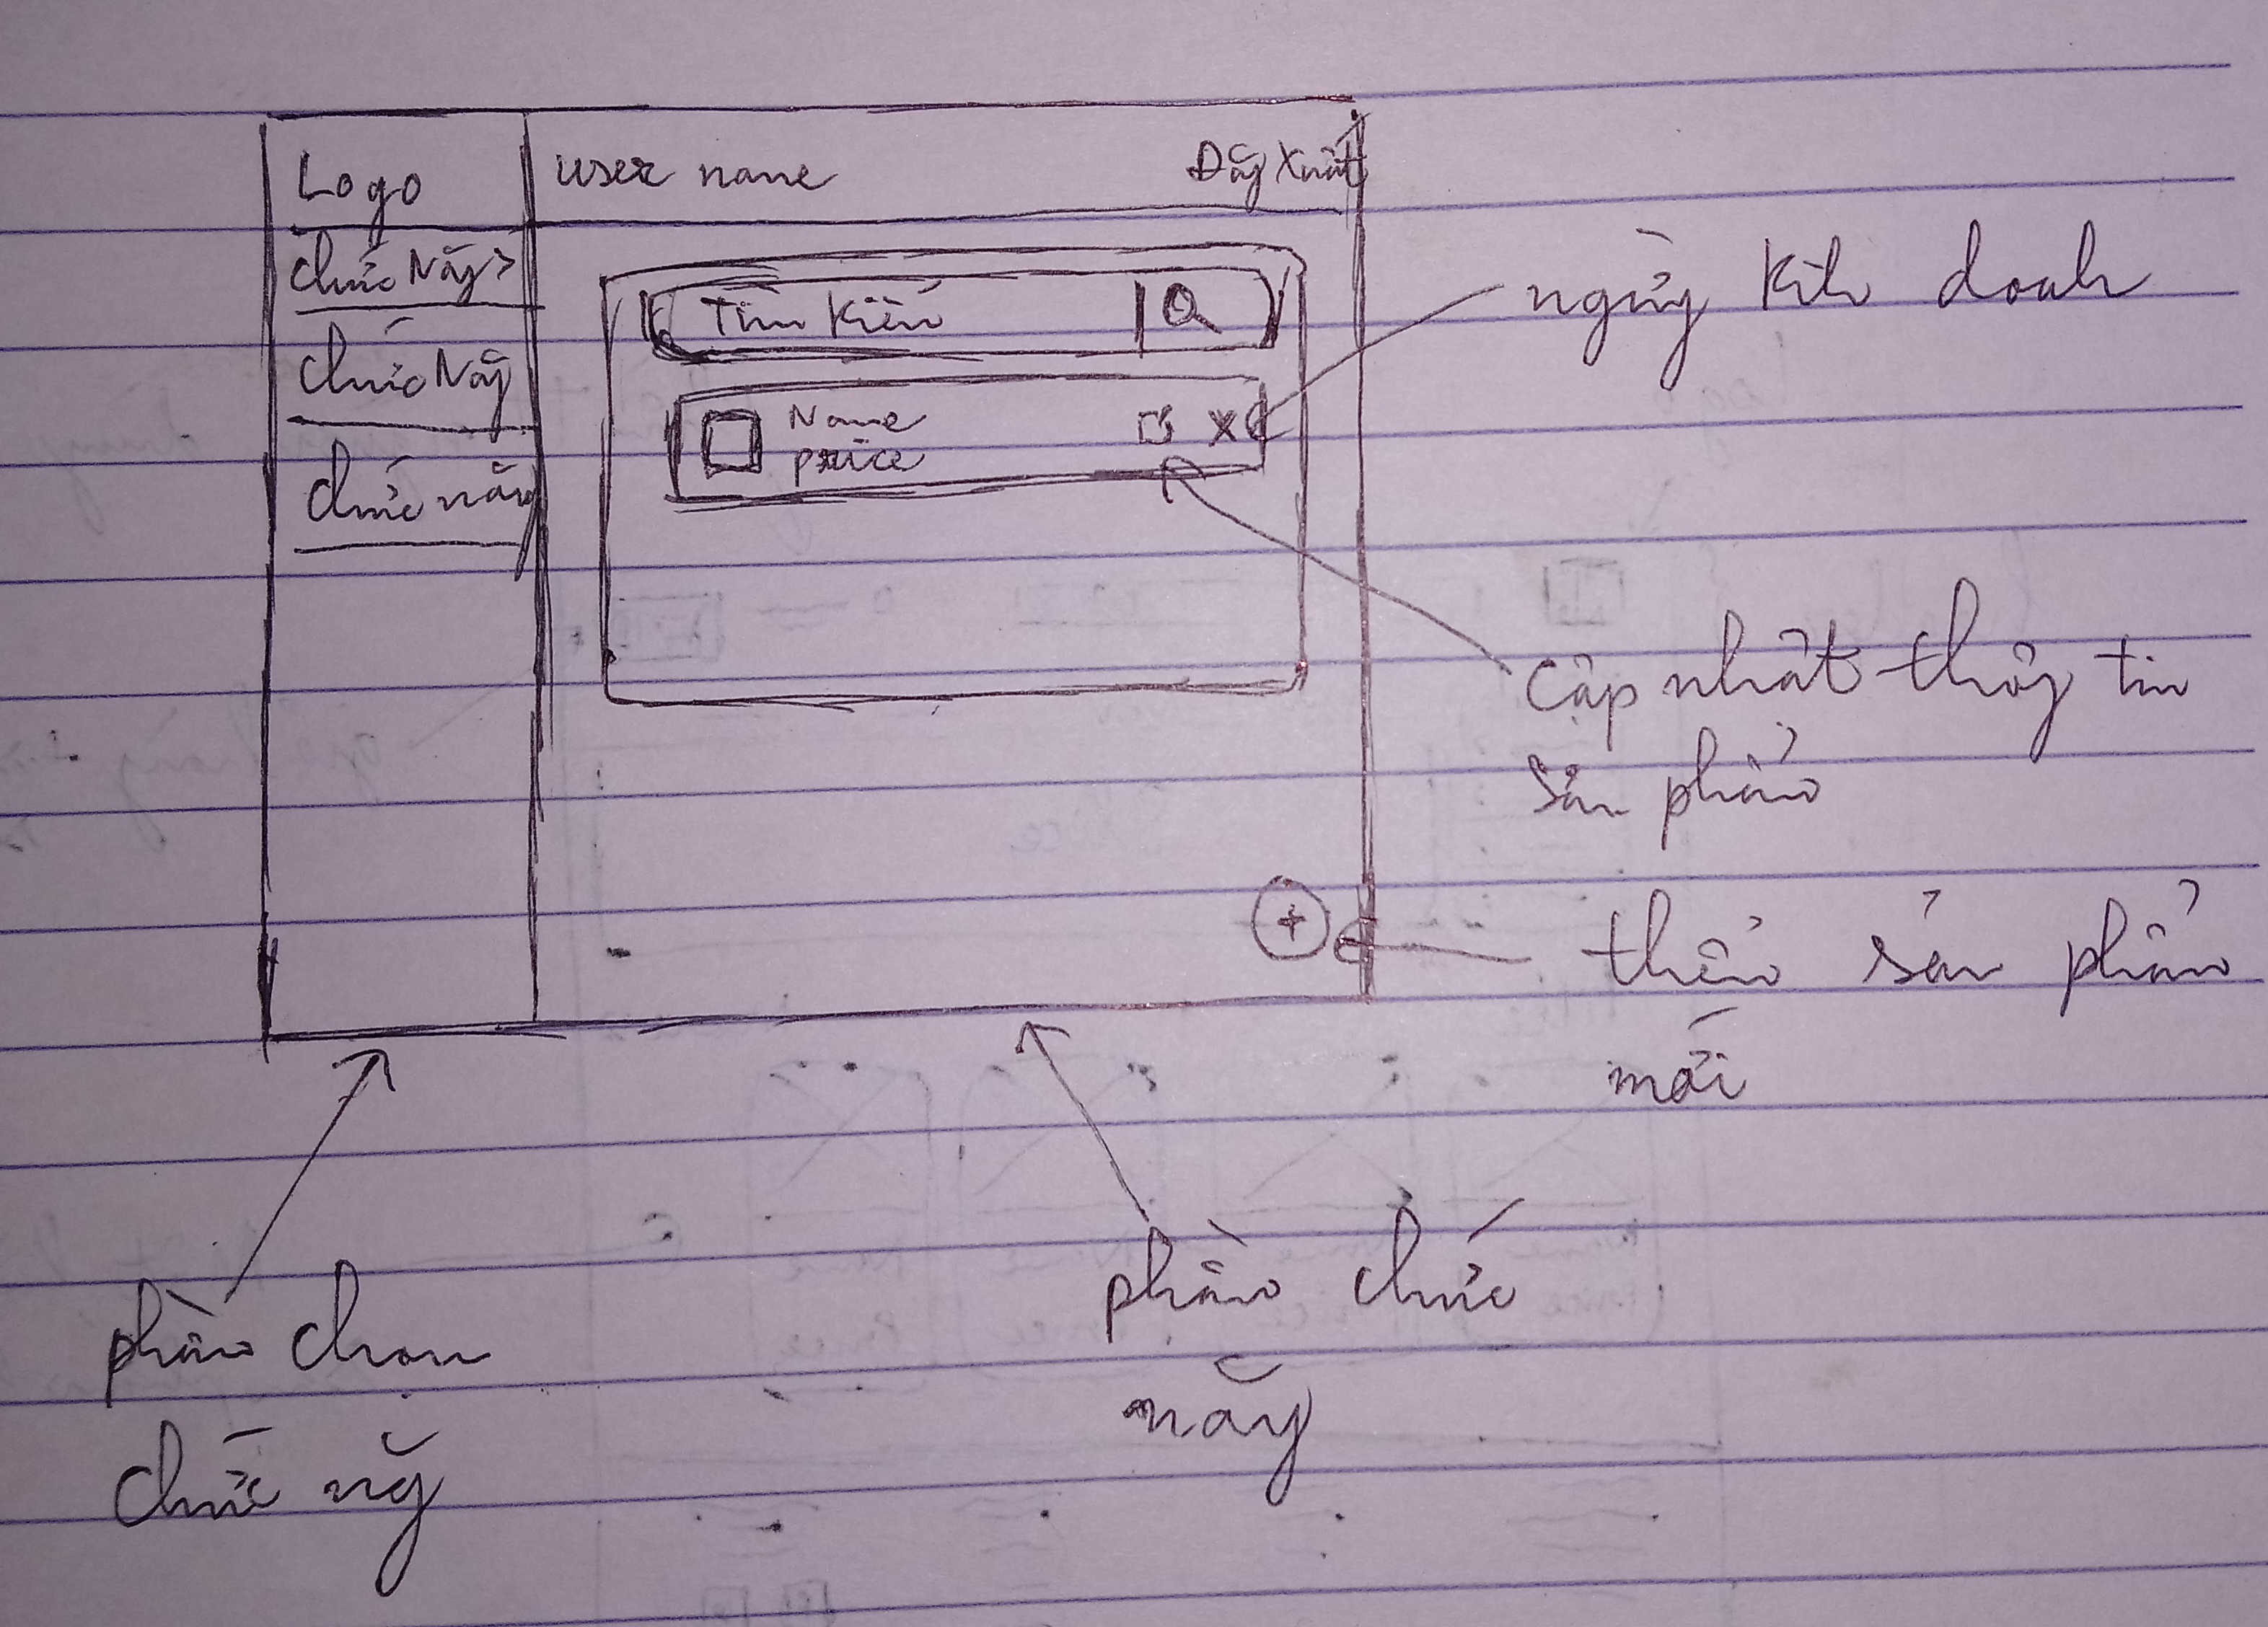
\includegraphics[width=\linewidth]{fig/p_dashboard.jpg}
            \caption{Nguyên mẫu thiết kế trang chủ}
        \end{figure}
\end{enumerate}
